\chapter{Problem Statement and Solver Methods}
\label{sec:solver}

In the following, the problem to optimize will be introduced an analyzed.
Although the thesis is not looking into finding the optimal solution, different solver strategies have to be introduced and compared to each other, as the utility function is not trivial and the differences are severe.
Their advantages and disadvantages will be shown.


\section{Utility Function}
\label{sec:utility_function}
As the aim for wireless communication networks is to maximize the achievable rate, we take the formulas derived in Section~\ref{sec:full_transf}, which describe the rates for each transmit-receive pair.
In order to get an utility function from the achievable rates, we stack them into the vector $\vec{r} = \begin{bmatrix}
r_1 \\ r_2 \\ \vdots \\ r_N
\end{bmatrix}$.

To optimize the rates, different approaches are possible.
\begin{itemize}
\item Optimize the minimum rate, i.e. $\text{max}\left(\text{min}(\vec{r})\right)$ (maxmin),
\item Optimize the mean rate, i.e. $\text{max}\left(\sum(\vec{r})\right)$ (maxsum), and
\item Optimize the maximum rate, i.e. $\text{max}\left(\text{max}(\vec{r})\right)$ (maxmax).
\end{itemize}

This is done using the LP-norm ($||\vec{r}||_p$)~\cite{wiki:lp_space}.
By setting $p = -\text{Inf}$, the "maxmin" method is achieved.
Setting $p = 1$, the "maxsum" method is applied and setting $p = +\text{Inf}$, the "maxmax" method is applied.
For all values in between, the utility function "tends" to optimize the maximum and minimum value respectively.

In the following we restrict ourselves to the "maxsum" method.
As the other methods easily can be applied and will lead to a similarly good result without loss of generality.

\subsection{Convexity of the Utility Function}
\label{sec:}

In the following the convexity of the utility function is analyzed.
This is done, because the choice of the solver depends on the shape of the utility function (e.g. in case of a concave utility function, a normal gradient search is sufficient to provide good results).

To do so, we analyze the utility function at different input values for the passive relays and at different input power values.
It is clear, that the function changes (heavily) for every channel realization.
Figure~\ref{fig:convex_3} shows two different channel realizations for the same input power and the same domain of two passive impedances.

\begin{figure}
\minipage{0.5\textwidth}
  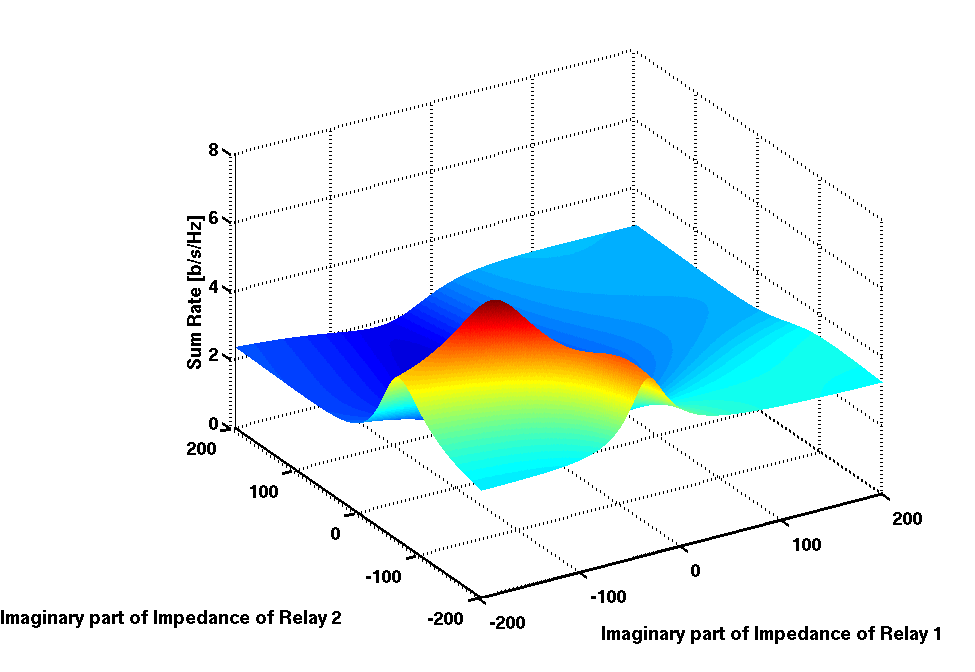
\includegraphics[width=\linewidth]{images/convex_1.png}
  %\caption{A really Awesome Image}
   \label{fig:convex_1}
\endminipage%\hfill
\minipage{0.5\textwidth}
  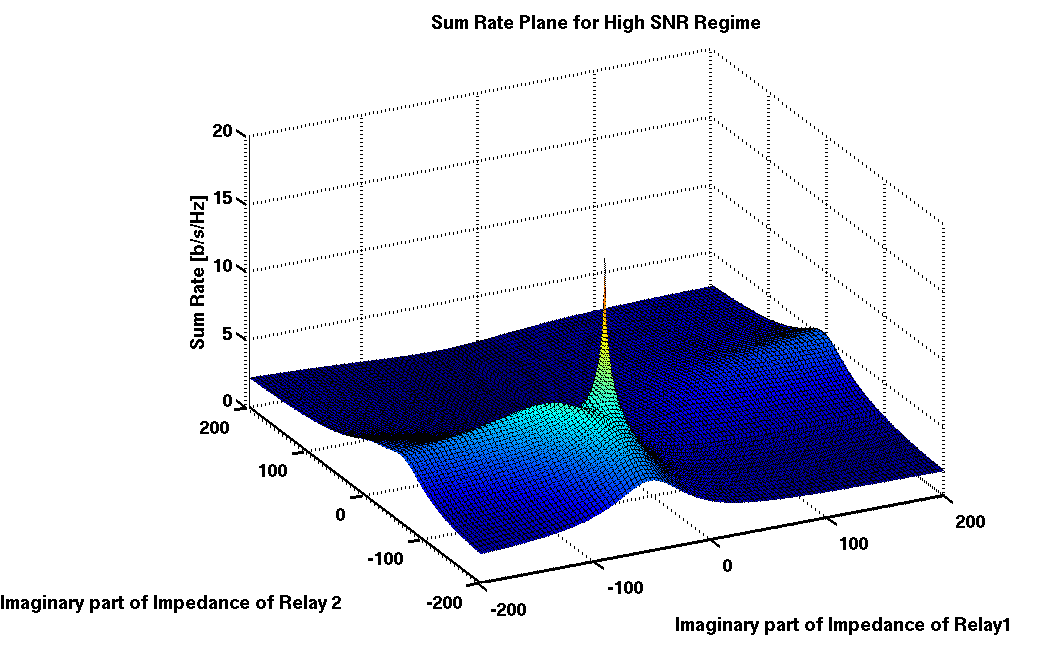
\includegraphics[width=\linewidth]{images/convex_2.png}
  %\caption{A really Awesome Image}
   \label{fig:convex_2}
\endminipage\hfill
\caption{The utility function for different imaginary relay impedances for two relays and two different channel realizations.}
   \label{fig:convex_3}
\end{figure}


\subsection{Dependency on the Input Power}
\label{sec:}

We will analyze now the utility function for different input powers.
In Figure~\ref{fig:utility_power1} and Figure~\ref{fig:utility_power2} we see the same channel realization for two different input powers.
Figure~\ref{fig:utility_power3} shows again the same channel realization at an input power close to the input power of Figure~\ref{fig:utility_power2}.

First we observe, that the optima in Figure~\ref{fig:utility_power1} and Figure~\ref{fig:utility_power2} lie at very different impedance values of the relays, therefore we can conclude, that an optimal solution for one input power does not necessarily lead to a good solution for a different input power solution.

Next we analyze the optima of Figure~\ref{fig:utility_power3} and Figure~\ref{fig:utility_power2}.
Here we can see again, that using the values from Figure~\ref{fig:utility_power3} in Figure~\ref{fig:utility_power2} will not lead to the best solution, however it would serves as a good initial value for a gradient search method.


\subsection{Difference of Local Optima}
\label{sec:}

Last, we want to look at the local optima we can possibly run into.
We see in Figure~\ref{fig:utility_power1}, that if we hit the local optimum at the left, the performance will be nearly the same as with the local optimum at the right.
However looking at Figure~\ref{fig:utility_power2}, we see that the difference of the local optimum before the peak and the peak itself is severe.
Therefore, we can not only try to run the optimization with one initialization, but instead, we need multiple initializations.

\subsection{Size of the Problem}
\label{sec:}

As we will discuss different solver approaches in the following Sections, a short description of the problem is given.
For each relay we use, we will have one variable ($N_\text{Rel}$), if we restrict the relays to the imaginary domain.
Allowing the relay to become lossy and therefore the impedance complex, the number of variables is doubled ($2\cdot N_\text{Rel}$).
Further for each receiver branch, we have a reciprocal (lossless) matching network, which can be optimized.
Therefore we have three elements per receiver branch or receiver antenna, respectively ($3\cdot N_\text{R}\cdot N_\text{Rx}$).
For a four user MIMO system with two receive antennas and five lossy relays per user, this would lead to a problem of size $N_\text{var} =  2\cdot 4\cdot 5 + 3\cdot 4\cdot 2 = 64$.

\section{Gradient Search}
\label{sec:grads_solver}

Despite this large number of variables and the non-convexity of the utility function, the first approach remains a gradient search.
Figure~\ref{fig:grad_search} shows the performance of the gradient search algorithm over the iterations.

\begin{figure}
\centering
  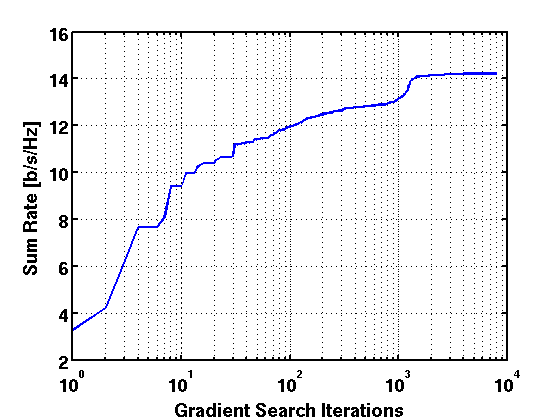
\includegraphics[width=0.7\linewidth]{images/rvsgradCnt_7rel_18dB_6.png}
\caption{The sum rate over the gradient search iterations.}
\label{fig:grad_search}
\end{figure}


\subsection{Initial Values}
\label{sec:grads_ini}

We try to overcome the non-pleasant properties of the problem with a larger number of initial guesses, so that the gradient search approach tends more towards a grid search optimization method.
The gradient search routine itself is then used as a refinement step of the grid search.
%(c.f. \cite{Adjashvili2012})

\begin{figure}[h]
\centering
  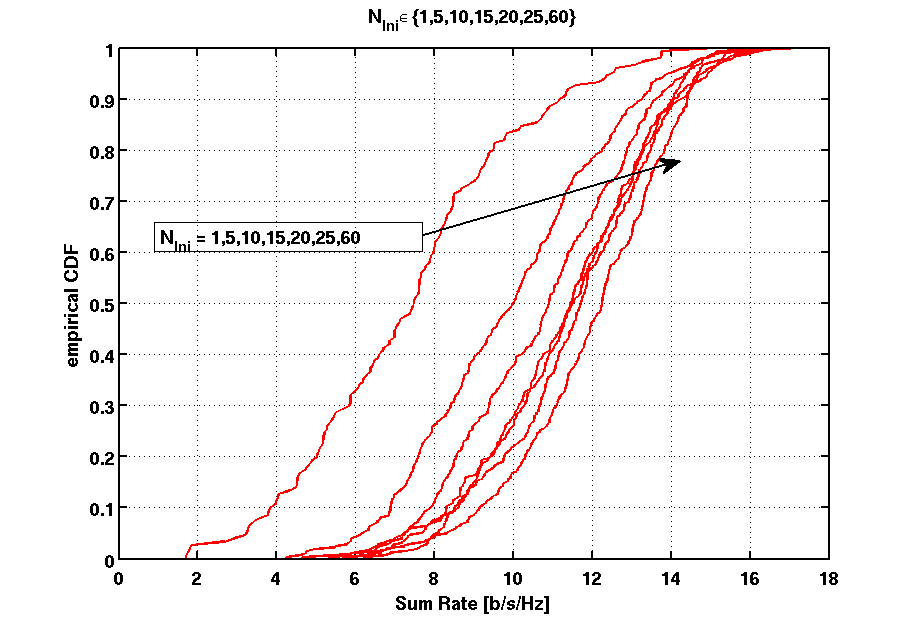
\includegraphics[width=0.8\linewidth]{images/Inicomparison_edited.png}
\caption{Comparison of the number of initial values used.}
\label{fig:ini_comp}
\end{figure}

Figure~\ref{fig:ini_comp} shows the empirical CDFs of the sum rate after the optimization, for different nuymber of initial values.
The initial values were drawn uniformly at random for $Z_{\text{Rel}}[i]\in[-600,600] j , \quad\forall i\in[1,N_{\text{Rel}}]$.

\subsubsection{Conclusion}
TO-DO

\subsection{Adaptive Step Size}
\label{sec:grads_stepsize}

The performance of the gradient search routine is improved by the use of an adaptive step size.
For each calculated gradient, the step taken into the direction of the gradient is increased until the new rate value is smaller than the previous calculated value.
Therefore the number of time-expensive gradient calculations is reduced immense.
If the starting step size immediately leads to a smaller sum rate value, the step size is decreased until it reaches a lower step-size-limit.
This lower step-size-limit serves together with a number of maximum gradient search iterations as the two terminating conditions of the whole algorithm.

PSEUDO-CODE 


\subsection{Conjugate Gradient}
\label{sec:grads_conjgrad}

As the gradient search performance still requires too many iterations, further improvements were made.
The shape of such complex problems can - in some cases - have the shape of a crest, where, with a unpleasant choice of the initial value, a pure gradient search routine might jump around the optimum, without improving a lot.
Conjugate gradient routines like "Fletcher-Reeves" or "Polak-Ribi\`{e}re" lead to a faster convergence, as they weight the gradient by the previous gradient. 

\subsubsection{Fletcher-Reeves}
\subsubsection{Polak-Ribi\`{e}re}
\begin{figure}[h]
\centering
  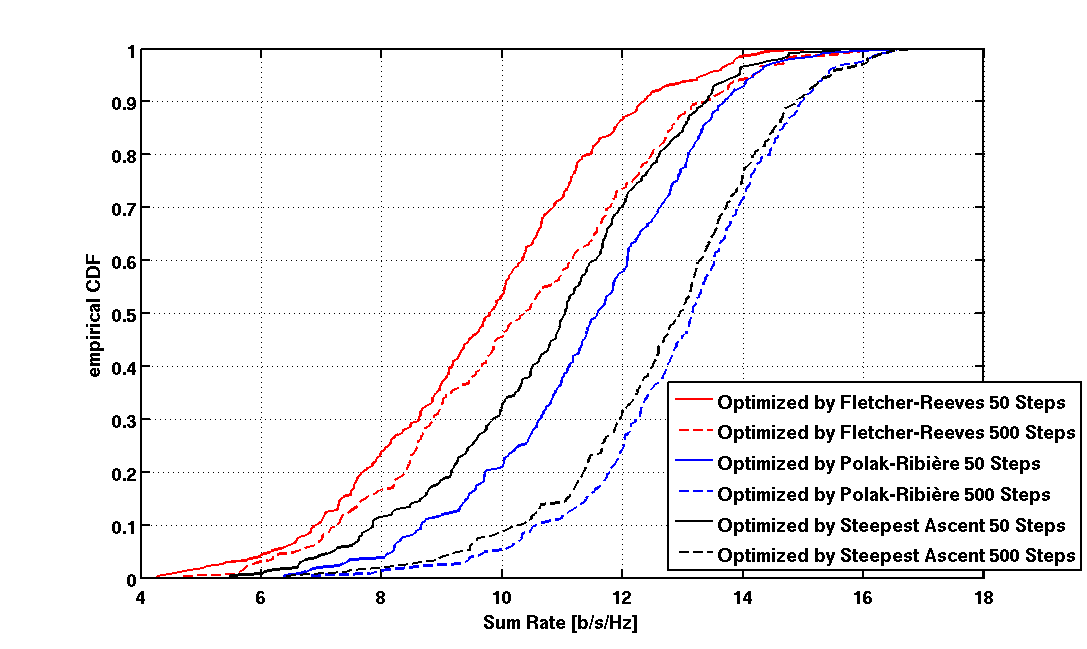
\includegraphics[width=0.7\linewidth]{images/Conjgradcomparison_edited.png}
\caption{Comparison between Steepest Ascent, Polak-Ribi\`{e}re, and Fletcher-Reeves.}
\label{fig:pr_fr_sa}
\end{figure}

\section{Heuristic Optimization Algorithms}
\label{sec:heuristic}

Due to the non convexity and the non trivial optimization problem, we further analyze (some) heuristic optimization methods.
In the following three heuristic algorithms will be introduced and analyzed by their performance.
They were chosen, because they already exist in the MATLAB library and do not require any strenuous implementation.

\subsection{Simulated Annealing}
\label{sec:sim_annealing}

Simulated Annealing was chosen as it is a method to solve optimization problems of large search space.
\cite{Ingber95}
\cite{matlab:simulann}
It is most often used for ...

\begin{figure}[h]
\centering
  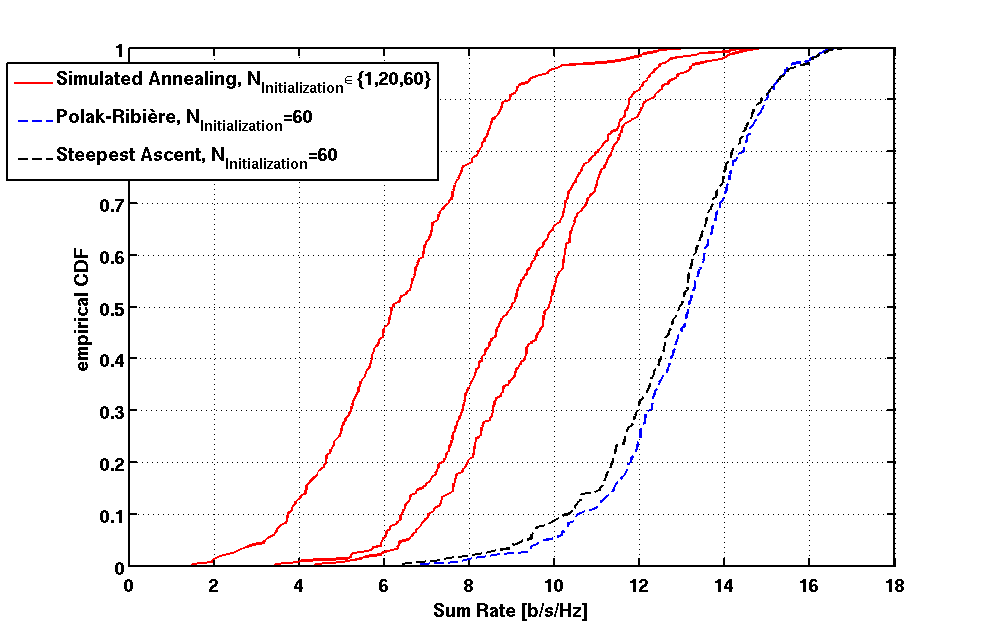
\includegraphics[width=0.7\linewidth]{images/Simannealcomparison.png}
\caption{Comparison of the Simulated Annealing algorithm for different number of initializations and the results from "Polak-Ribi\`{e}re" and "Steepest Ascent" gradient searches.}
\label{fig:pr_fr_sa}
\end{figure}


\subsection{GlobalSearch}
\label{sec:globals}

The other two heuristic optimization algorithms are GlobalSearch (GS) and MultiStart (MS).
They are very similar to each other, the only difference is the choice of the starting values.
As MultiStart requires the number of initialization values, GS generates trial points on its own~\cite{matlab:gloabls}.

\begin{figure}[h]
\centering
  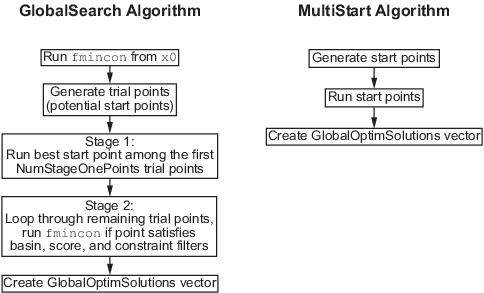
\includegraphics[width=0.7\linewidth]{images/global_algorithm.png}
\caption{Schematics of the GlobalSearch and MultiStart algorithms~\cite{matlab:gloabls}.}
\label{fig:globals_scheme}
\end{figure}
Figure~\ref{fig:globals_scheme} shows the schematics of GS and MS.

\begin{figure}[h]
\centering
  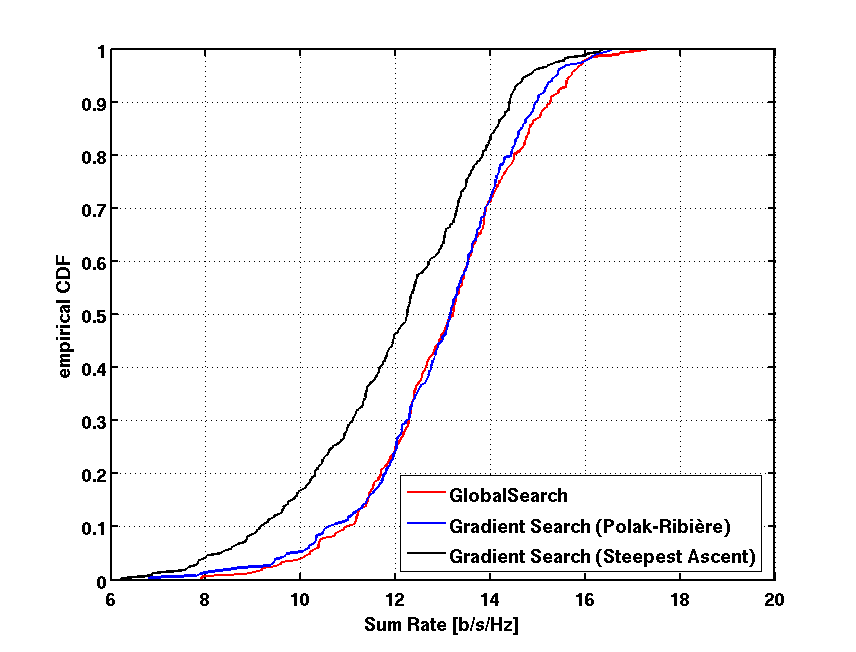
\includegraphics[width=0.7\linewidth]{images/Globalscomparison_edited.png}
\caption{Performance of the GlobalSearch algorithm in comparison to the previous results.}
\label{fig:globals}
\end{figure}

\section{Further Algorithm Improvements}

\subsection{Optimization of the Interference Function}

A further approach to optimize the gradient search routine is a good initial guess.
The problem of the sum rate maximization is reduced only to the description of the interference.
Therefore the number of variables can be reduced by a factor of two third for the matching network, as the interference function

REFERENCE

only requires the input impedance of the matching network.
This reduced problem has size of $N_\text{var} =  2\cdot N_\text{Rel}+2\cdot N_\text{R}\cdot N_\text{Rx} = 2\cdot 4\cdot 5 + 2\cdot 4\cdot 2 = 56$, for the same settings as above.
The factor 2 from the matching network variables comes from the fact, that with pure imaginary elements in the matching network, any complex value of the input impedance can be achieved.

\begin{figure}[h]
\centering
  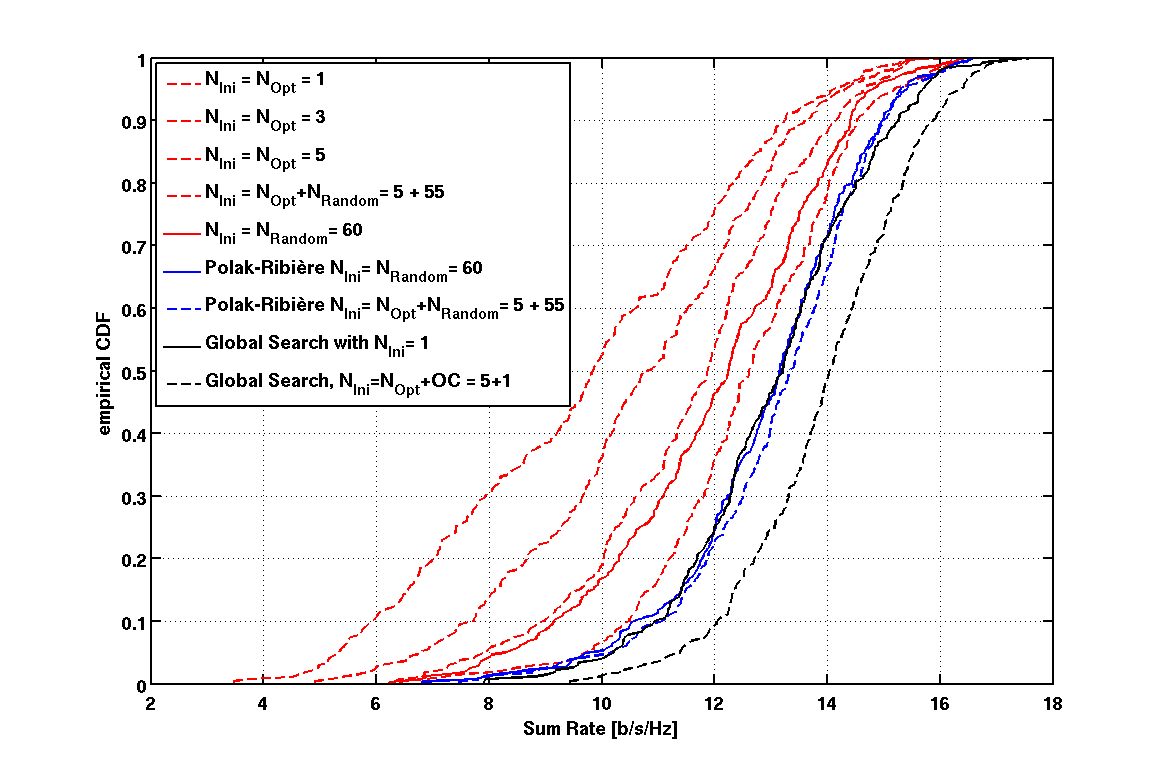
\includegraphics[width=0.8\linewidth]{images/Inioptcomparison_edited.png}
\caption{Comparison of the number of initial values used.}
\label{fig:ini_comp}
\end{figure}

\subsection{Post Refinement of GlobalSearch by Gradient Search}
Stepwise improvement of the relays.


\subsection{Stepwise Relay Improvements}
Stepwise improvement of the relays.







